\subsection{Sample scatter touched against commit - } 
\begin{figure}[!htbp]
  \centering 
\begin{minipage}[b]{0.45\textwidth}
    \centering
    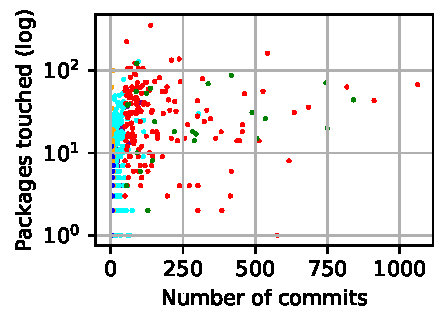
\includegraphics[width=\textwidth]{ sections/results/graph/sample_scatter_touched_against_commit.packages.sample.first.pdf }
    \vskip 5pt
    {\small Packages}
    \label{ figure.35.700000000000095 }
\end{minipage}%
\hfill
\begin{minipage}[b]{0.45\textwidth}
    \centering
    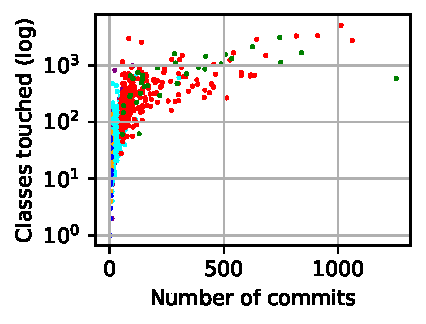
\includegraphics[width=\textwidth]{ sections/results/graph/sample_scatter_touched_against_commit.classes.sample.first.pdf }
    \vskip 5pt
    {\small Classes}
    \label{ figure.35.8000000000001 }
\end{minipage}%
\hfill
  \vfill
\begin{minipage}[b]{0.45\textwidth}
    \centering
    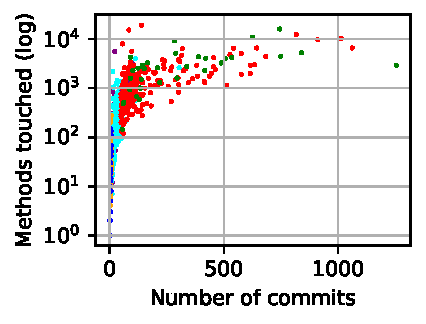
\includegraphics[width=\textwidth]{ sections/results/graph/sample_scatter_touched_against_commit.methods.sample.first.pdf }
    \vskip 5pt
    {\small Methods}
    \label{ figure.35.9000000000001 }
\end{minipage}%
\hfill
\caption{Scatter plots of the log total number of components touched (y-axis) against the number of commits (x-axis) made by samples of developers capped at 203 sustained later joiners from six (6) categories: \color{Blue}Transient Founder (Blue, 63), \color{Purple}Moderate Founder (Purple, 40), \color{Green} Sustained Founder (Green, 34), \color{Orange} Transient Later Joiner (Orange, 203), \color{Cyan}Moderate Later Joiner (Cyan, 203), \color{Red} Sustained Later Joiner (Red, 203). \color{Black}} 
\end{figure}
\newpage 
